\documentclass[10pt]{article}
\usepackage{listings}
\usepackage{xcolor}
\usepackage{graphicx}
\usepackage{pythonhighlight}
\usepackage[left = 2cm,right = 2cm,top = 3 cm,bottom = 3cm]{geometry}
 \lstset{columns = fixed,
 numbers = left,
 frame = none,
 backgroundcolor = \color[RGB]{240,244,245},
 keywordstyle = \color[RGB]{0,0,255},
 numberstyle = \footnotesize\color{darkgray},
 commentstyle = \it\color[RGB]{255,96,96},
 stringstyle = \rmfamily\slshape\color[RGB]{255,0,255},
 showstringspaces = false,
 language=C++,
 }
\begin{document}
  \title{Study Report}
  \author{Shuo Xu}
  \maketitle
 \begin{abstract}
 
 In this week, I finished the first two courses of deeplearning. I've already used tensorflow and have known some functions,in this report I will do some review and learn the latex at the same time.

 Unfortunately, I didn't install it on my manjaro which caused my manjaro couldn't boot again, in the end I lost all my files. I spent nearly a whole day to salve the problem but failed, maybe I will come back Ubuntu next week...Good job, Nvidia.
 \end{abstract}
 \begin{center}
 \section{Review}
 \begin{flushleft}
 
 The first class is mainly talked some basic knowledge which is not difficult to understand. The following are the review of the second class, Improving Deep Neural Networks: Hyperparameter tuning, Regularization and Optimization. It mainly talk about the adjustment and optimization method of Neural Networks.
 \end{flushleft}
 \end{center}
 \subsection{Train/Dev/Test sets}
 \begin{itemize}
\item train sets : used to train network parameters
\item develpoment sets : verify and select the best model
\item test sets : test the performance of the best algorithm
\end{itemize}

  The recommended allocation ratio is as follows:\\

\begin{center}
\begin{tabular}{|c|c|c|c|}
\hline
\cline{1-2}
Data quantity   & Train   & Dev     &Test \\
\hline
1,000-10,000    & 60\%    & 20\%    &10\%  \\
                & 70\%    & 30\%    & 0   \\
\hline
1,000,000       & 98\%    & 1\%      & 1\%  \\
\hline
 $>$1,000,000   & 99.5\%  & 0.25\%   &0.25\%   \\
                & 99.5\%  & 0.4\%    &0.1\%   \\
\hline
\end{tabular}  
\end{center}

  \subsection{Bias/Variance}
  
  \begin{flushleft}
  
    Bias and variance are two very important concepts and problems to be solved in machine learning. High bias means that the prediction ability of the model is not enough, which shows that the training error is large. While high variance means that the generalization ability of the model is insufficient, which shows that the test error is large. And, of course, they might be at the same time. The following pictures are some examples. 
     
  \end{flushleft}
    
  
  \begin{center}
    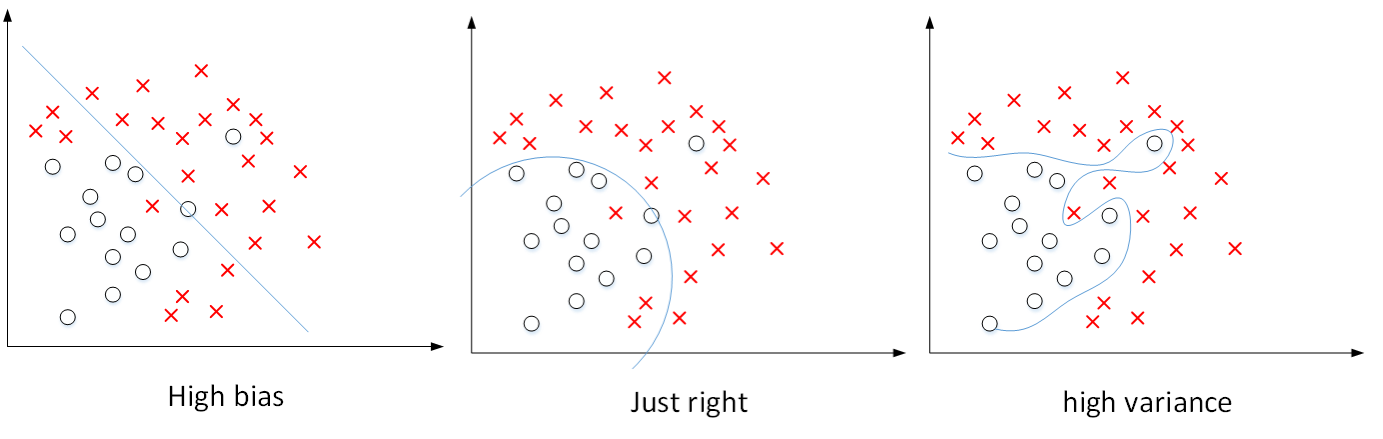
\includegraphics[scale=0.4]{bias.jpg}
    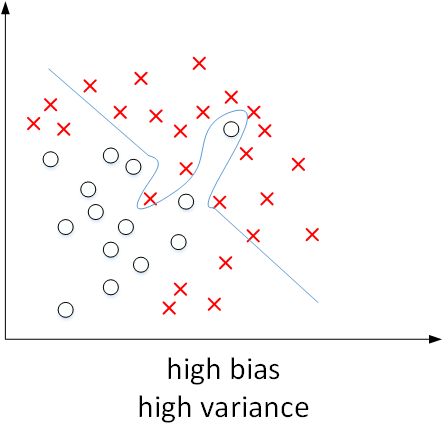
\includegraphics[scale=0.4]{sametime.jpg}
  \end{center}
  
  The video also mentioned the method to solve the two problems.\\
  
  
  For high bias:
  
  
  1. deeper and wider networks



2. for longer training



3. better optimization methods



4. better network structure\\


For high variance:


1. more data



2. regularization



3. better network structure


The video takes a lot of time to explain the details of these methods, but I think some is unnecessary.

 \subsection{Regularization}
 \begin{itemize}
 \item{L2 regularization}
 \begin{flushleft}
 For Logistic regression:\\
 $$J_{R} = \frac{1}{m}\sum_{i=1}^{m}(y^{(i)}log(a^{[l](i)})+(1-y^{(i)})log(1-a^{[L](i)}) + -\frac{1}{m}\frac{\lambda}{2}\sum_{l}\sum_{k}\sum_{j}W_{kj}^{[1]2}$$
$$\frac{d}{dW}(\frac{1}{2}\frac{\lambda}{m}W^{2})=\frac{\lambda}{m}W $$

 "lambda" is reserved word in python, can't use it to name a variable.\\ In L2 regularization, we can't set $\lambda$ a large value, otherwise the result will be too smooth, which could cause high bias.
 \end{flushleft}
 
 
 \item Dropout
 \begin{flushleft}
 By setting a variable called "keep-prob", close some units in every layer. Use this method we can make our neural network not sensitive to some distinctive neuron as it can be closed anytime. So it is useful to reduce variance. The following is an example of how to use "keep-prob" of Python.
 
 \begin{python}
 D[1] = np.random.rand(A.shape[0], A.shape[1])
 D[1] = D[1] < keep-prob
 A[1] = np.multiply(A[1], D[1])
 A[1] = A1 / keep-prob
 
 # backward
 dA[1] = np.multiply(dA[1], D[1])
 dA[1] = dA[1] / keep-prob
 \end{python}
  Normally we don't set "keep-prob" for the input layer. If we need, it will be a number close to one.  Many of the first successful implementations of drop outs were to computer vision. Because in computer vision we have enough data, a very large number.
 \end{flushleft}
 
 \item Other regularization methods
 \begin{flushleft}
 By some method like add noise, we can get some new data from our old data. After we get more training examples, we can reduce over fitting in our neural network.
 \end{flushleft}
 \end{itemize}
 
 \subsection{Normalizing inputs}
 \begin{flushleft}
 This is a way to speed up our training.It has three steps:
 $$\mu=\frac{1}{m} \sum_{i=1}^{m}X^{(i)}$$
 $$\sigma^{2} = \frac{1}{m}\sum_{i=1}^{m}(X^{(i)})^2$$
 $$X:=\frac{X-\mu}{\sigma^{2}}$$     
 \begin{center}
 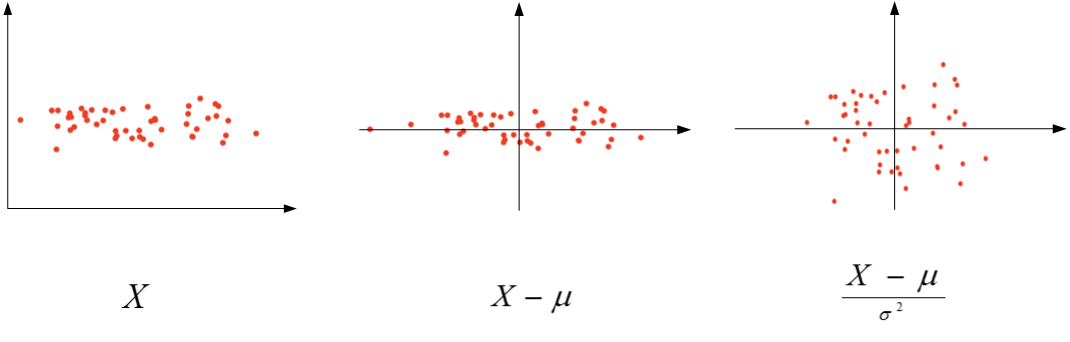
\includegraphics[scale=0.6]{guiyi.jpg}
 \end{center}
 
 \end{flushleft}
 
 
 
 \begin{center}
 \section{Leetcode}
 \end{center}
 \subsection*{Gas Station}
 \begin{itemize}
 \item Problem
 \begin{flushleft}
 There are N gas stations along a circular route, where the amount of gas at station i is gas[i].

You have a car with an unlimited gas tank and it costs cost[i] of gas to travel from station i to its next station (i+1). You begin the journey with an empty tank at one of the gas stations.

Return the starting gas station's index if you can travel around the circuit once in the clockwise direction, otherwise return -1.
 
 \end{flushleft}
 \item Solution
 \begin{flushleft}
 At first my solution is go through the gas array, judge every gas station by my helper function. It is clear and easy to implement, but it runs too slow. After deeply thinking, I found I did a lot of unless work. As long as the total number of gas is bigger than the total number of cost, we can finish the journey. For a  gas station, if the cost is bigger than gas number, the station can't be the start. \\
 So, I have a new solution only use one loop. Set variable start to represent the start number, total to calculate the difference of gas and cost of every gas station and store the sum for judgement, sum to store the temporary total value for update. The initial value of them are all zero. Traversing each data, calculate the difference between gas-number and cost and add it to the total and sum. If sum is less than zero, make the value of sum become 0 and make the value of start become i+1.\\
 After the loop, if total is less than zero the function will return -1,else it will return start.
 \end{flushleft}
 \item Code
 \begin{lstlisting}
 class Solution {
public:
    int canCompleteCircuit(vector<int>& gas, vector<int>& cost) {
        for(int i=0;i<gas.size();i++){
            if(helper(gas,cost,gas[i]-cost[i],i,i+1))
                return i;
        }
        return -1;
    }

    bool helper(vector<int>& gas,vector<int>& cost,int tank,int index,int now){
        if(tank<0)
            return false;
        if(now==gas.size())
            now=0;
        if(now==index)
            return true;
        return helper(gas,cost,tank+gas[now]-cost[now],index,now+1);
    }
};
 \end{lstlisting}
 better solution:
 \begin{lstlisting}
 class Solution {
public:
    int canCompleteCircuit(vector<int>& gas, vector<int>& cost) {
        int total = 0, sum = 0, start = 0;
        for (int i = 0; i < gas.size(); ++i) {
            total += gas[i] - cost[i];
            sum += gas[i] - cost[i];
            if (sum < 0) {
                start = i + 1;
                sum = 0;
            }
        }
        return (total < 0) ? -1 : start;
    }
};
\end{lstlisting}
 \end{itemize}
 
 \begin{center}
 \section{Others}
 \end{center}
 \begin{flushleft}
  I nearly spent the main time to write this report, learn the latex and review the knowledge from the video at the same time. What I had wrote is only a little part of the videos. I think if I want to write all the things by latex, I should write latex everyday instead of only one day, and it is necessary. 
  
  I tried to write a MLP program like the given "True\_MLP", but I found the part of backward propagation is too difficult. Softmax is a very useful function but I didn't know it until the day before yesterday. Now I have known tensorflow, next week I will try again.
  
  There is also a problem about tensorflow. As Linux is not friendly to the dGPU, why tensorflow mainly runs on linux especially on Ubuntu? 
 \end{flushleft}

\end{document}